
% ----- Consignes exo xx ----- %
\begin{td-exo}[Flots --- 3pts]\,\\ % xx
    Calculer un flot maximal sur le réseau de transport ci-dessous, commençant par une augmentation de flot le long du chemin \(sadbep\).
    En expliquant comment l'obtenir, donner une coupe minimale du réseau.

    \ffigbox[\FBwidth]{%
\caption{\centering Réseau de transport initial}\label{Fig:exam_blanc_ex_1_1}
}{
    \fbox{
        \begin{tikzpicture}[scale=1, main node/.style={circle, draw, fill=blue!20, inner sep=1pt, font=\scriptsize, minimum size=6mm}]
            % les sommets initiaux
            \node[main node] (s) at (-3,0) {\(s\)};
            \node[main node] (p) at (3,0) {\(p\)};

            \node[main node] (a) at (-1,2) {\(a\)};
            \node[main node] (b) at (-1,0) {\(b\)};
            \node[main node] (c) at (-1,-2) {\(c\)};

            \node[main node] (d) at (1,2) {\(d\)};
            \node[main node] (e) at (1,0) {\(e\)};
            \node[main node] (f) at (1,-2) {\(f\)};

            % les arcs avec capacités
            \draw[-{Stealth}] (s) -- node[above left] {\(4\)} (a);
            \draw[-{Stealth}] (s) -- node[above] {\(5\)} (b);
            \draw[-{Stealth}] (s) -- node[below left] {\(4\)} (c);

            \draw[-{Stealth}] (a) -- node[above] {\(5\)} (d);

            \draw[-{Stealth}] (b) -- node[above] {\(6\)} (e);
            \draw[-{Stealth}] (b) -- node[left] {\(9\)} (f);

            \draw[-{Stealth}] (c) -- node[below] {\(1\)} (f);

            \draw[-{Stealth}] (d) -- node[above right] {\(2\)} (b);
            \draw[-{Stealth}] (d) -- node[above right] {\(3\)} (p);

            \draw[-{Stealth}] (e) -- node[right] {\(9\)} (c);
            \draw[-{Stealth}] (e) -- node[below right] {\(9\)} (p);

            \draw[-{Stealth}] (f) -- node[below right] {\(1\)} (p);
        \end{tikzpicture}
    }
}
\end{td-exo}

% ----- Solutions exo xx ----- %
\iftoggle{showsolutions}{
	\begin{td-sol}[]\,\\ % xx
		Exercice solution
	\end{td-sol}
}{}


% ----- Consignes exo xx ----- %
\begin{td-exo}[Indépendant dans les subcubiques --- 5pts]\,\\ % xx
    Un graphe \(G = (V,E)\) est dit \defemph{subcubique} si tous ses sommets ont degré au plus 3, c'est à dire si \(\forall v\in V, \mathsf{deg}_G(v) \leq 3\).
    Le but de l'exercice est de donner des bornes sur \(\alpha(G)\), la taille du plus grand ensemble indépendant (ou stable) de \(G\) en fonction de \(n\), le nombre de sommets de \(G\).
    \begin{enumerate}
        \item On commence par fournir une borne inférieure pour \(\alpha(G)\).
        \begin{enumerate}
            \item Montrer que si \(x\) est un sommet de \(G\) et \(I\) un indépendant de \(G \setminus \left( x\cup N_G(x) \right)\) alors \(I \cup \{x\}\) est un indépendant de \(G\).
            \item En déduire, par récurrence sur \(n\), que tout graphe subcubique à \(n\) sommets admet un indépendant de taille au moins \(\lceil \frac{n}{4} \rceil\).
        \end{enumerate}

        \item On suppose maintenant que \(G\) est cubique (c'est à dire \(\forall v\in V, \mathsf{deg}_G(v) = 3\)) et on va établir une borne supérieure pour \(\alpha(G)\).
        \begin{enumerate}
            \item soit \(X\) un indépendant de \(G\). En fonction de la taille de \(X\), calculer le nombre d'arêtes, noté \(e(X, \ol{X})\), entre \(X\) et son complémentaire.
            \item En déduire que \(|X| \leq |\ol{X}|\) puis que \(|X| \leq \lfloor \frac{n}{2} \rfloor\).
        \end{enumerate}

        \item Donner deux exemples de graphes cubiques \(G_1\) et \(G_2\) sur \(n\) sommets tels que \(\alpha(G_1) = \frac{n}{4}\) et \(\alpha(G_2) = \frac{n}{2}\). Si possible, vous donnerez des exemples pour \(n\) arbitrairement grand.
    \end{enumerate}
\end{td-exo}

% ----- Solutions exo xx ----- %
\iftoggle{showsolutions}{
	\begin{td-sol}[]\,\\ % xx
		Exercice solution
	\end{td-sol}
}{}


% ----- Consignes exo xx ----- %
\begin{td-exo}[Couplage max --- 3pts]\,\\ % xx
    Dans le graphe suivant, appliquer l'algorithme d'Edmonds pour calculer un couplage maximum, en sachant que le couplage \(\left\{ be, ci, hp \right\}\) a déjà été précalculé. Au cours de votre déroulement d'algorithme, vous devrez, à au moins une reprise, contracter un blossom.

    \ffigbox[\FBwidth]{%
\caption{\centering Graphe avec couplage \(\{be, ci, hp\}\) précalculé}\label{Fig:exam_blanc_ex_3_1}
}{
    \fbox{
        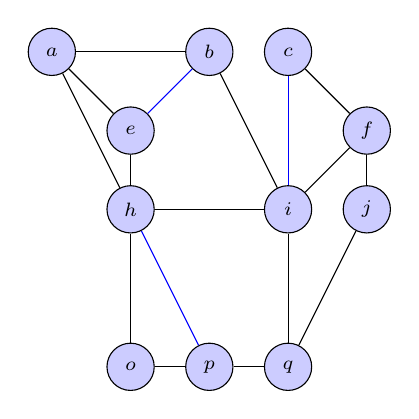
\begin{tikzpicture}[scale=1, main node/.style={circle, draw, fill=blue!20, inner sep=1pt, font=\scriptsize, minimum size=6mm}]
            % les sommets initiaux
            \node[main node] (a) at (-2,2) {\(a\)};
            \node[main node] (b) at (0,2) {\(b\)};
            \node[main node] (c) at (1,2) {\(c\)};

            \node[main node] (e) at (-1,1) {\(e\)};
            \node[main node] (f) at (2,1) {\(f\)};

            \node[main node] (h) at (-1,0) {\(h\)};
            \node[main node] (i) at (1,0) {\(i\)};
            \node[main node] (j) at (2, 0) {\(j\)};

            \node[main node] (o) at (-1, -2) {\(o\)};
            \node[main node] (p) at (0, -2) {\(p\)};
            \node[main node] (q) at (1, -2) {\(q\)};

            % les aretes
            \draw[] (a) -- (b);
            \draw[] (a) -- (e);
            \draw[] (a) -- (h);

            \draw[draw=blue] (b) -- (e);
            \draw[] (b) -- (i);

            \draw[] (c) -- (f);
            \draw[draw=blue] (c) -- (i);
            \draw[] (e) -- (h);

            \draw[] (f) -- (i);
            \draw[] (f) -- (j);

            \draw[] (h) -- (i);
            \draw[] (h) -- (o);
            \draw[draw=blue] (h) -- (p);

            \draw[] (i) -- (q);

            \draw[] (j) -- (q);

            \draw[] (o) -- (p);

            \draw[] (p) -- (q);
        \end{tikzpicture}
    }
}
\end{td-exo}

% ----- Solutions exo xx ----- %
\iftoggle{showsolutions}{
	\begin{td-sol}[]\,\\ % xx   
        Exercice solution
	\end{td-sol}
}{}


% ----- Consignes exo xx ----- %
\begin{td-exo}[Miam! --- 5pts]\,\\ % xx
    Trois étudiants affamés, nommés \(E_1, E_2\) et \(E_3\), se retrouvent pour manger 6 pizzas, notées \(P_1, \ldots, P_6\).
    Chaque étudiant veut manger 2 pizzas exactement. Les étudiants ont les contraintes alimentaires suivantes:
    \begin{itemize}
        \item \(E_1\) qui déteste les champignons, ne veut manger que les pizzas \(P_1, P_4\) et \(P_5\).
        \item \(E_2\) qui est allergique au chorizo, ne veut manger que les pizzas \(P_2, P_5\) et \(P_6\).
        \item \(E_3\) qui ne digère pas les anchois, ne veut manger que les pizzas \(P_1, P_2, P_3\) et \(P_6\).
    \end{itemize}
    On souhaite savoir si il est possible de répartir les 6 pizzas afin de satisfaire les choix des étudiants.
    \begin{enumerate}
        \item Construire le graphe biparti \(H_{(E, P)}\) défini sur \(\left\{P_1, \ldots, P_6\right\} \cup \left\{E_1, E_2, E_3\right\}\) et dont les arêtes sont \(\{P_i E_j : \) si \(E_j\) veut manger la pizza \(P_i\}\).
        \item Quelle structure souhaite-t-on trouver dans \(H_{(E, P)}\) pour garantir une solution au problème?
        \item Une \defemph{copie} d'un sommet \(x\) dans un graphe \(G\) est un sommet \(y\) non-adjacent à \(x\) et dont le voisinage est identique à celui de \(x\). A partir du graphe \(H_{(E, P)}\), on construit le graphe \(H_{(E, P)}'\) en ajoutant une copie pour chaque sommet \(E_i\). Sans preuve, quelle structure souhaite-t-on trouver dans \(H_{(E, P)}'\) pour garantir que les trois étudiants peuvent se répartir les six pizzas en respectant leurs choix?
        \item Résoudre le problème (en utilisant un algorithme du cours \(\ldots\)).
        \item Plus généralement, soit \(k\geq 2\) fixé, le \defemph{centre} d'un graphe biparti complet \(K_{1, k}\) est le sommet de ce graphe qui n'est pas une feuille. 
        Etant donné un graphe biparti \(G = ((A, B), E)\), on souhaite déterminer si \(G\) peut être (sommet-)\~partitionné en graphes \(K_{1, k}\) dont les centres sont tous dans \(A\). 
        Donner un algorithme de résolution en temps polynomial pour ce problème. Prouver la validité de votre algorithme.
    \end{enumerate}
\end{td-exo}

% ----- Solutions exo xx ----- %
\iftoggle{showsolutions}{
	\begin{td-sol}[]\,\\ % xx
		Exercice solution
	\end{td-sol}
}{}


% ----- Consignes exo xx ----- %
\begin{td-exo}[Graphes auto-complémentaires --- 4pts]\,\\ % xx
    Un graphe \(G\) est dit \defemph{auto-complémentaire} si \(G\) est isomorphe à son complémentaire \(\ol{G}\).
    \begin{enumerate}
        \item Justifier que \(P_4\) et \(C_5\) sont auto-complémentaires.
        \item Montrer que tout graphe auto-complémentaire est connexe.
        \item En notant \(n\) le nombre de sommets de \(G\), calculer le nombre d'arêtes d'un graphe auto-complémentaire en fonction de \(n\).
        \item En déduire que \(n \equiv 0 \text{ ou } 1 \mod 4\).
        \item Soit \(G\) un graphe auto-complémentaire et \(P\) un chemin de longueur 3 (c'est à dire avec 4 sommets).
        On note \(G'\) le graphe obtenu depuis \(G \cup P\) en reliant le premier et le dernier sommet de \(P\) à tous les sommets de \(G\).
        Montrer que \(G'\) est auto-complémentaire.
        \item En déduire que pour tout \(n\) avec \(n \equiv 0 \text{ ou } 1 \mod 4\), il existe un graphe auto-complémentaire à \(n\) sommets.
    \end{enumerate}
\end{td-exo}

% ----- Solutions exo xx ----- %
\iftoggle{showsolutions}{
	\begin{td-sol}[]\,\\ % xx
		Exercice solution
	\end{td-sol}
}{}